% GeomTok — "Compression Is Not Modelability"
% ACL/ARR submission. Compile with pdfLaTeX: acl_latex -> bibtex -> acl_latex x2.
% Change [review] -> [final] for camera-ready, or -> [preprint] for a non-anonymous arXiv version.
\documentclass[11pt]{article}
\usepackage[review]{acl}

\usepackage{times}
\usepackage{latexsym}
\usepackage[T1]{fontenc}
\usepackage[utf8]{inputenc}
\usepackage{microtype}
\usepackage{inconsolata}
\usepackage{graphicx}
\usepackage{booktabs}
\usepackage{amsmath}
\usepackage{amssymb}

\graphicspath{{figures/}}

% --- Anonymity-aware switches (driven by the acl class option) ---------------
% [review]  -> author auto-hidden as "Anonymous ACL submission"; anonymized URL.
% [preprint]/[final] -> real author shown; real repository URL.
\makeatletter
\ifacl@anonymize
  \newcommand{\resourceurl}{\url{https://anonymous.4open.science/r/geomtok}\ (anonymized for review)}
\else
  \newcommand{\resourceurl}{\url{https://github.com/Stayhealthy88/GeomTok}}
  \hypersetup{pdfauthor={Gyuwook Byun}, pdftitle={Compression Is Not Modelability}}
\fi
\makeatother
% -----------------------------------------------------------------------------

\title{Compression Is Not Modelability:\\ A Controlled Study of Tokenization Units for Vector Graphics}

% In [review] the author is auto-hidden as "Anonymous ACL submission" (acl.sty);
% the name below appears only in [preprint]/[final]. Confirm affiliation + email
% before camera-ready.
\author{Gyuwook Byun \\
  Independent Researcher \\
  \texttt{igotthepower0128@gmail.com}}

\begin{document}
\maketitle

\begin{abstract}
Large language models tokenize vector graphics (SVG) the way they tokenize prose, shredding a coordinate like \texttt{150.5} into characters that carry no spatial meaning. We ask a narrow, falsifiable question: does the \emph{unit} a model reads geometry in change downstream modeling? We introduce \textbf{GeomTok}, a geometry-native SVG tokenizer (commands, shapes, and a zero-vocabulary fixed-point coordinate codec), and \textbf{GeomTok-Eval}, a render-based intrinsic \emph{tokenizer} protocol decoupled from any generator. Under a controlled tokenizer-swap on an identical small transformer, geometric primitive tokens model held-out icons 18--26\% better (held-out NLL) than a domain-trained text BPE---a result that replicates across two corpora (icons and emoji) and does not vanish with scale (the gap \emph{widens then plateaus} over a $10\times$ parameter range)---and, under identical plain sampling, a text tokenizer generates 0\% renderable SVG versus 84\% for GeomTok. Our central result is a controlled counterexample, in the graphics setting, to the assumption that intrinsic compression predicts downstream modeling---a relationship already shown non-monotonic for text by PathPiece \citep{schmidt2024pathpiece}: more compression never reliably helps. We release the protocol, fair baselines, and a set of adversarially-verified negative results---including retracted claims---as a methodological contribution. We scope all model-level claims to the small-model, sample-efficient regime.\footnote{Code, the GeomTok-Eval protocol, per-experiment data-split manifests, and the full negative-results ledger are available: \resourceurl.}
\end{abstract}

\section{Introduction}
Vector graphics underlie nearly every digital interface: icons, logos, UI components, charts, and maps. Yet generative models remain unreliable at producing them---circles fail to close, rectangles drift off-grid, coordinates land in the wrong place. A widely cited cause is \textbf{tokenization}: a coordinate \texttt{150.5} is fragmented by a text tokenizer into \texttt{1}, \texttt{50}, \texttt{.}, \texttt{5}, destroying the fact that it denotes a point in space \citep{xing2024llm4svg}.

Recent work attacks this with geometry-aware tokenization---HiVG \citep{hivg2026} groups SVG commands into geometry-constrained two-level (atomic and segment) tokens; OmniSVG \citep{omnisvg2025} folds each \((x,y)\) into a single grid token; StrokeNUWA \citep{strokenuwa2024} learns a VQ codebook. These works establish that geometry-aware tokens compress SVG and improve fidelity. \textbf{What the field has not isolated is the downstream consequence of the tokenization \emph{unit} itself}, under a controlled, generator-decoupled comparison against fair baselines. That gap is the subject of this paper. We treat it as a \emph{tokenizer-evaluation} question in the lineage of the fixed-model tokenizer-swap \citep{ali2024tokenizer,lotz2025} and the text-domain finding that fewer tokens need not mean better downstream behavior \citep{schmidt2024pathpiece}.

A note on rigor, up front. An earlier version of this work asserted a $7.6\times$ compression headline, a training benefit from geometry-aware embedding initialization, and an adaptive-quadtree coordinate scheme. Each was falsified by a control we ran---a matched-vocabulary baseline, a matched-embedding-norm baseline, and a real-data comparison, respectively (\S\ref{sec:controls}). We report these retractions as part of the contribution; the surviving claims are the ones that survived adversarial verification.

We make three contributions:
\begin{enumerate}
\item \textbf{GeomTok}---a geometry-native tokenizer whose fixed-point coordinate codec adds zero vocabulary, achieving 100\% parse and bounded-error round-trip and $3.54\times$ compression at matched vocabulary (\S\ref{sec:method}, \S\ref{sec:efficiency}).
\item \textbf{Compression is not modelability}---under a controlled, generator-decoupled tokenizer-swap, primitive tokens model and generate best, while the most-compressed variant models and generates \emph{worst}---a clean counterexample, for vector graphics, to the assumption that intrinsic compression predicts downstream quality (\S\ref{sec:downstream}--\S\ref{sec:generation}).
\item \textbf{GeomTok-Eval and a negative-results discipline}---a render-based intrinsic protocol that resists gaming, released alongside adversarially-verified retractions of our own earlier claims (\S\ref{sec:eval}, \S\ref{sec:controls}).
\end{enumerate}

\section{Related Work and Positioning}
\textbf{Geometry-aware SVG tokenization.} HiVG \citep{hivg2026} is the closest prior work: it groups SVG commands into geometry-constrained two-level (atomic/segment) tokens and trains with a hierarchical mean-noise embedding initialization. OmniSVG \citep{omnisvg2025} merges \((x,y)\) into single grid tokens; LLM4SVG \citep{xing2024llm4svg} adds semantic tokens to an LLM vocabulary; StrokeNUWA \citep{strokenuwa2024} learns a VQ-Stroke codebook (lossy); InternSVG \citep{internsvg2025} unifies SVG understanding/editing/generation with SVG-specific special tokens. We do \textbf{not} claim to be first to operate over geometric primitives---HiVG and, in the protein domain, GeoBPE \citep{geobpe2026} precede us. Our novelty is comparative and methodological: to our knowledge the first controlled char-BPE / primitive / learned-merge / structure-constrained comparison on real SVG under a single fixed model, plus a generator-decoupled, render- and value-grounded protocol. A concurrent line takes the opposite route---modeling SVG numbers continuously rather than as discrete tokens \citep{ogezi2026cnm}---without isolating the tokenization unit; we discuss it as an orthogonal challenger in the Limitations.

\textbf{Compression vs.\ downstream.} That intrinsic compression does not monotonically predict downstream quality is established for \emph{text} by PathPiece \citep{schmidt2024pathpiece} and by \citet{lotz2025}, and the fixed-model tokenizer-swap protocol originates in \citet{ali2024tokenizer}. In the \emph{raster-image} domain, the relationship is shown to be capacity-dependent for discrete autoregressive generation \citep{raster2024compress}---more-compressed stage-1 latents can \emph{help} smaller stage-2 models even as reconstruction worsens. We contribute the first \emph{vector-graphics} instance, isolated by a controlled tokenizer-swap and grounded in render fidelity---a setting where, in contrast to that raster-image result, more compression never reliably helps and on icons monotonically hurts.

\textbf{Numeric tokenization.} xVal \citep{xval2023}, FoNE \citep{fone2025}, and a regression-like number-token loss \citep{ntl2025} study how to encode numbers in transformers. Our fixed-point codec (\S\ref{sec:codec}) is a deliberately simple instance---a quadtree leaf grid reinterpreted as a base-64 numeral system---chosen to isolate the substrate effect, not to advance numeric encoding.

\textbf{Name disambiguation.} ``GeomTok'' is unrelated to \emph{GeoToken} \citep{ghasemi2025geotoken}, which tokenizes an image-geolocalization \emph{output} into S2 geographic cells; we operate on SVG geometry primitives. Render-based generator-agnostic SVG metrics also exist for generated \emph{code structure} \citep{zhu2026svgmetrics}; GeomTok-Eval instead targets the \emph{tokenizer} and adds value-level fidelity and cross-vocabulary bits/icon (\S\ref{sec:eval}).

\section{Method: GeomTok}
\label{sec:method}
\subsection{Pipeline}
SVG $\rightarrow$ \textbf{parse} (flatten transforms + group inheritance, normalize viewBox, drop non-rendered \texttt{defs}/\texttt{clipPath}) $\rightarrow$ \textbf{quantize} (uniform $64\times64$ coordinate grid; \S\ref{sec:codec}) $\rightarrow$ \textbf{tokenize} (commands, shapes, coordinates) $\rightarrow$ optional \textbf{grammar-constrained decode} (an FSA guarantees valid SVG; used only when a downstream application wants a hard validity guarantee---it is \emph{not} used in any experiment below). We adopt the uniform grid as the shipped default; the comparison against an adaptive scheme that justifies this choice is reported with the other controls in \S\ref{sec:controls}.

The vocabulary is 5{,}561 tokens: \textbf{5{,}461 coordinate tokens} plus ${\sim}100$ structural tokens (5 special, 8 command, 4 shape, 4 continuity, 16 curvature, 11 spatial), with remaining IDs held as reserved ranges for forward-compatible extension. The coordinate tokens cover quadtree levels 0--6; the level-6 leaf grid is $64\times64=4{,}096$ cells, which the codec below reuses as a numeral system.

\subsection{Scalar fixed-point codec}
\label{sec:codec}
A scalar such as a radius or gap must be encoded without inflating the vocabulary. We reinterpret the level-6 grid ($64\times64=4096$ cells) as a base-64 numeral system, so a scalar $v\in[0,\text{canvas})$ maps to a single coordinate token $q_x\cdot64+q_y$. This adds \textbf{zero vocabulary} and bounds scalar error to $\text{canvas}/(4096{-}1)/2\approx0.04$px. Counts (e.g.\ a repeat count) use an exact integer variant with lossless round-trip up to 4095. (An earlier $(v,v)$ encoding through the 2-D quadtree produced up to $17.5$px error and broke repeat counts; full account in \S\ref{sec:controls}.)

\subsection{Token levels}
\label{sec:levels}
L1 emits geometric primitives (commands + coordinates) and is the default. L2 applies learned (frequency-based) merges over L1; L3 adds spatial-relation tokens. As \S\ref{sec:downstream} shows that more aggressive merging is \emph{not} downstream-optimal, \textbf{L1 is the default and compression is opt-in}, documented as a trade-off rather than a free win.

Beyond bare commands and coordinates, L1 inserts two families of \emph{auxiliary geometric markers}: per-anchor \textbf{continuity} flags (smooth/cusp/\ldots) and quantized \textbf{curvature} bins on curve segments. These are not free---on the held-out svg-icons split they are \textbf{24.2\% of all L1 tokens} (continuity 18.6\%, curvature 5.6\%; mean 120.8 tok/icon, of which 29.2 are markers). Because they inflate sequence length, their inclusion is a deliberate design choice that an ablation must justify rather than assume. It does not: \S\ref{sec:efficiency} shows the markers are derivable (zero reconstruction effect) yet \emph{raise} held-out NLL by ${\sim}12\%$, so we recommend a \textbf{lean L1} that omits them. We retain them in the as-shipped configuration used by \S\ref{sec:merges}--\S\ref{sec:generation}, which makes those results a conservative reading of the geometric advantage.

\section{GeomTok-Eval}
\label{sec:eval}
A geometric tokenizer needs intrinsic metrics that (a) work on real, path-only icons, (b) resist gaming, and (c) are computable without a GPU. GeomTok-Eval reports:
\begin{itemize}
\item \textbf{Parse / round-trip rate}---fraction of a corpus that tokenizes and reconstructs.
\item \textbf{Token efficiency}---tokens/icon \emph{and} encoding bits/icon ($=$ tokens $\times \log_2$ vocab), the latter making cross-vocabulary comparison fair. We distinguish this \emph{intrinsic} encoding-bits/icon from the \emph{held-out NLL} bits/icon of \S\ref{sec:downstream}, a trained-model quantity.
\item \textbf{Value-level fidelity}---per-coordinate $L_2$ error after a tokenize$\rightarrow$detokenize round-trip, extended to path coordinates (negative and exponent numbers, positional matching) so it does not return $\infty$ on path-only icons.
\item \textbf{Render fidelity}---SSIM and ink-IoU between rasterized original and reconstruction (resvg, 64--256px).
\end{itemize}
We motivate the protocol with a concrete failure it catches: an earlier ``structural score'' awarded a perfect 1.000 to random token sequences while scoring ground truth 0.987---a metric that ranked tokenizers backwards. GeomTok-Eval is \emph{generator-decoupled} (it scores the tokenizer's reconstruction, not a generator's output), which is what makes random-sequence gaming impossible.

\section{Experiments}
\label{sec:experiments}
All experiments use the public StarVector svg-icons benchmark (monochrome, path-centric). Tokenizer-swap experiments train an identical 2.5M-parameter decoder-only transformer (a vanilla model with no GeomTok-specific embedding) on each tokenizer's stream---the only variable is the tokenizer \citep{ali2024tokenizer}. The domain text baseline is a SentencePiece BPE trained on SVG text at vocab 5{,}561 (a \emph{fair} baseline; GPT-4's cl100k, at 100k vocab and not domain-trained, is reported only as a reference). Crucially, generation (\S\ref{sec:generation}) uses \textbf{identical plain top-$k$ sampling for every arm with no grammar constraint}, so the geometric arm receives no FSA-validity advantage. \textbf{All baselines are our own reimplementations under a single fixed backbone}---char-BPE, the HiVG-inspired and boundary-constrained merge rules (\S\ref{sec:merges}), and the continuous-coordinate head (Limitations)---not the original released systems; this is by design, since the contribution is the \emph{controlled} tokenizer-swap, which requires every arm to share one backbone and corpus.

\begin{figure*}[t]
\centering
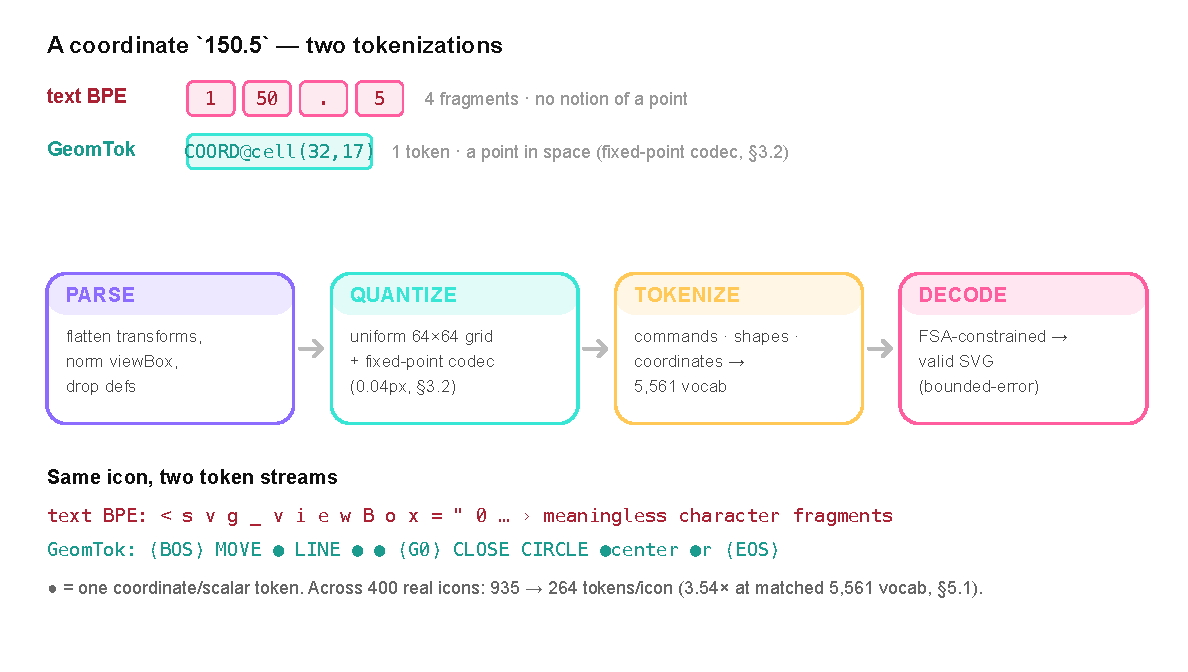
\includegraphics[width=\textwidth]{fig1_pipeline.pdf}
\caption{The GeomTok pipeline. A coordinate \texttt{150.5} is shredded by text BPE into 4 fragments versus one GeomTok coordinate token, with the same-icon token-stream contrast below.}
\label{fig:pipeline}
\end{figure*}

\subsection{Tokenizer efficiency (intrinsic)}
\label{sec:efficiency}
On 400 real icons (Table~\ref{tab:efficiency}), GeomTok-L1 reaches $3.54\times$ compression over the domain char-BPE at matched vocabulary.

\begin{table}[t]
\centering
\small
\begin{tabular}{lrrr}
\toprule
Scheme & tok/icon & bits/icon & vs.\ BPE \\
\midrule
GPT-4 cl100k (ref.) & 2021 & 33{,}580 & $0.46\times$ \\
Domain char-BPE & 935 & 11{,}636 & $1.00\times$ \\
\textbf{GeomTok-L1} & \textbf{264} & \textbf{3{,}287} & $\mathbf{3.54\times}$ \\
GeomTok-L1 + BPE & 151 & 1{,}925 & $6.21\times$ \\
\bottomrule
\end{tabular}
\caption{Intrinsic efficiency, 400 real icons. Encoding bits/icon $=$ tokens $\times \log_2$ vocab.}
\label{tab:efficiency}
\end{table}

GeomTok-L1's coordinate fidelity is \textbf{1.78px mean / 3.37px max} on a 300px canvas (within the analytic bound), with render SSIM \textbf{0.929}---the fidelity cost of the $3.54\times$ compression (the round-trip is geometric and bounded-error, not lossless). Hand-crafted shape tokens (L2) fire on \textbf{0\%} of real icons and add nothing.

\textbf{Auxiliary-marker ablation (the markers do not earn their cost---a negative result).} L1 emits per-anchor continuity and per-segment curvature markers (\S\ref{sec:levels}), 24.2\% of all L1 tokens. First, they are \textbf{derivable, not load-bearing}: the detokenizer parses but never uses them (reconstruction reads only command and coordinate tokens), and stripping them is \textbf{byte-identical on 57/57 held-out icons}---zero fidelity cost. Second, on the tokenizer-swap protocol (980 train / 205 test, 3 seeds, 25 epochs) stripping them \emph{improves} held-out NLL from $687.2\pm2.0$ to $602.4\pm2.7$ bits/icon ($-84.8$, ${\approx}12\%$, far beyond seed noise) \emph{and} shortens sequences ($120.8\rightarrow91.6$ tokens/icon). A model spends ${\sim}12\%$ of its budget predicting tokens it can already derive and that the decoder ignores. This is the mechanism of \S\ref{sec:downstream} read in reverse: removing \emph{zero-information} tokens compresses \emph{and} helps, whereas BPE merges compress by raising per-token entropy and hurt---it is \textbf{what} you compress, not how much. We therefore recommend a \textbf{lean L1}; the \S\ref{sec:merges}--\S\ref{sec:generation} results use full L1, making the L1-vs-text gap a \emph{conservative} lower bound.

\subsection{Learned vs.\ structure-constrained merges}
\label{sec:merges}
Applying an identical greedy BPE to three substrates at a matched merge budget (train 1{,}200 / test 400; Table~\ref{tab:merges}):

\begin{table}[t]
\centering
\small
\begin{tabular}{lrrrr}
\toprule
Budget & char & L1 & L1 bnd. & L1 HiVG-st. \\
\midrule
0 & 4893 & 264 & 264 & 264 \\
1000 & 824 & \textbf{172} & 222 & 236 \\
\bottomrule
\end{tabular}
\caption{Tokens/icon at matched merge budget. ``L1'' $=$ unconstrained learned merges; ``bnd.'' $=$ boundary-constrained; ``HiVG-st.'' $=$ a HiVG-inspired, command-rooted geometry-constrained merge rule applied to our L1 stream.}
\label{tab:merges}
\end{table}

Encoding bits/icon @1000: char $7245 \gg$ L1 $1687 <$ boundary $1890 <$ HiVG-style $1934$---identical ranking. \textbf{At matched budget, unconstrained learned merges use 27\% fewer tokens than the HiVG-inspired structure-constrained rule (172 vs.\ 236)}: the constraint forbids cross-command repeated patterns that unconstrained BPE exploits. We compare the \emph{merge rule}---a command-rooted, geometry-constrained pairing applied to our L1 stream---not HiVG's full representation; this isolates the constraint's effect on a shared substrate. This is an intrinsic-compression comparison at fixed budget, not a claim of downstream superiority for L1+BPE (see \S\ref{sec:downstream}).

\subsection{Downstream: the compression--modelability split}
\label{sec:downstream}
Identical 2.5M model, real icons (1{,}045 train / 213 test), tokenizer swapped, 3 seeds, held-out NLL bits/icon, lower is better (Table~\ref{tab:downstream}).

\begin{table}[t]
\centering
\small
\begin{tabular}{lrr}
\toprule
Arm & tok/icon & NLL bits/icon ($n{=}3$) \\
\midrule
char-BPE & 159 & $775\pm6$ \\
L1 + learned BPE & 59 & $666\pm2$ \\
\textbf{GeomTok-L1} & 104 & $\mathbf{576\pm4}$ \\
\bottomrule
\end{tabular}
\caption{Downstream modeling. Absolute NLL is comparable only \emph{within} a panel (panels below use different splits/lengths); cross-panel claims rest only on the \emph{direction} of the L1-vs-baseline gap. The gap here is overwhelming (Welch $t\approx-48$ for char-BPE vs.\ L1).}
\label{tab:downstream}
\end{table}

Two findings; both gaps are large relative to seed variance (std 2--6 bits, against gaps of 90--199 bits):
\begin{enumerate}
\item \textbf{Geometric primitive tokens are the best downstream substrate in this regime}---26\% better modeling than a domain text tokenizer (576 vs.\ 775).
\item \textbf{Compression does not reliably predict modelability}---L1+BPE compresses $1.8\times$ more than L1 (59 vs.\ 104 tokens) yet models \emph{worse} (666 vs.\ 576), because merges raise per-token entropy (11.3 vs.\ 5.6 bits/token). The most-compressed tokenizer is not the best to learn from.
\end{enumerate}

\textbf{Budget sweep (a curve, not a point).} Sweeping the merge budget $N$ on L1 (1{,}000 train / 200 test, $n{=}2$): as $N$ rises, tokens/icon falls monotonically ($105\rightarrow65$ at $N{=}0,250,500,1k,2k$) while held-out NLL rises monotonically ($608\rightarrow680$). Every added merge compresses more and models worse; pure L1 is the downstream optimum (Figure~\ref{fig:scatter}).

\begin{figure}[t]
\centering
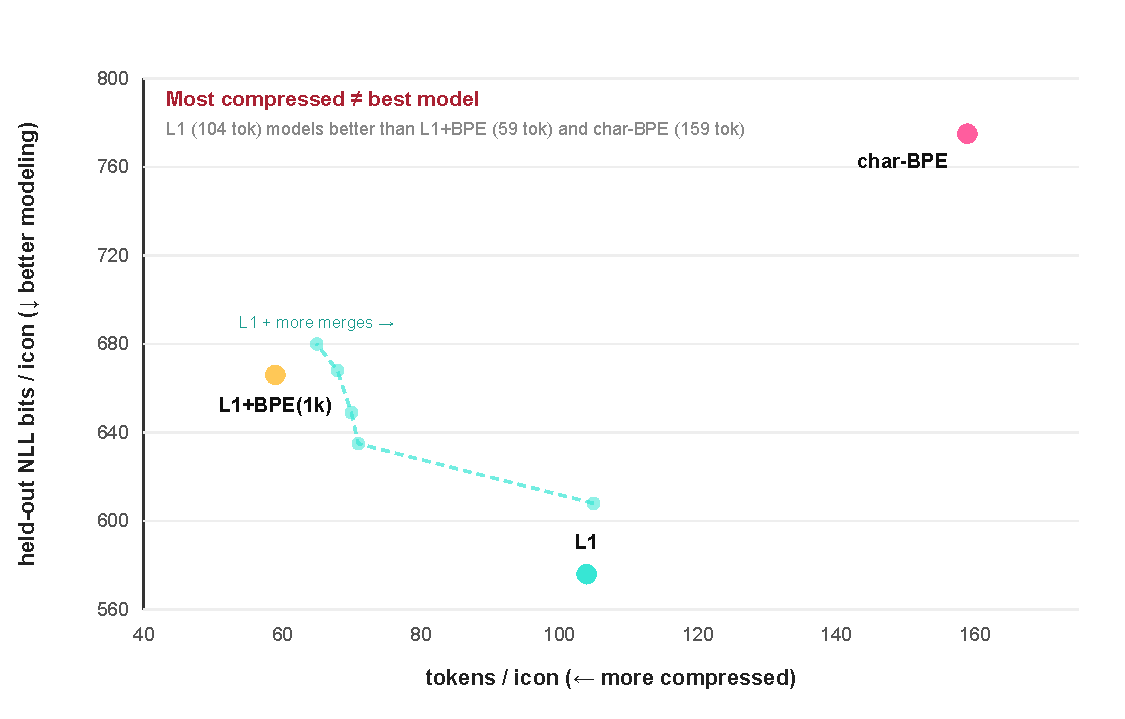
\includegraphics[width=\columnwidth]{fig2_compression_modelability.pdf}
\caption{Compression--modelability scatter: x $=$ tokens/icon (intrinsic compression), y $=$ held-out NLL (modelability). The most-compressed tokenizer is not the best to learn from; the L1 budget-sweep trend is overlaid.}
\label{fig:scatter}
\end{figure}

\textbf{Capacity trend (the gap does not vanish with scale).} Running the L1-vs-L1+BPE(1k) swap at four sizes (Table~\ref{tab:capacity}), L1 wins at every size and the gap \emph{widens then plateaus} ($35\rightarrow47\rightarrow62\rightarrow62$), rather than shrinking toward zero as a small-model artifact would. The gap stops widening by 4.6M, so we claim persistence, not unbounded growth; whether it holds at 100M--1B is future work. (Single seed per size; treated as a trend.)

\begin{table}[t]
\centering
\small
\begin{tabular}{lrrr}
\toprule
params & L1 NLL & L1+BPE NLL & gap \\
\midrule
0.9M & 754 & 788 & 35 \\
2.2M & 708 & 755 & 47 \\
4.6M & 661 & 723 & 62 \\
9.3M & 634 & 696 & 62 \\
\bottomrule
\end{tabular}
\caption{Capacity trend. L1 wins across a $10\times$ parameter range.}
\label{tab:capacity}
\end{table}

\textbf{Second corpus (the primary claim replicates).} Repeating the swap on \textbf{svg-emoji} (colored, 401 train / 48 test, $n{=}3$), the \emph{primary} substrate result replicates strongly---both geometric arms crush text BPE: L1 $1117\pm27$ and L1+BPE $1086\pm44$ vs.\ char-BPE $1356\pm5$ (18\% better than text). The \emph{specific} compression direction does not transfer: on emoji L1+BPE (1086) is statistically tied with L1 (1117) (gap $31<$ combined std ${\sim}52$), rather than worse as on svg-icons. Across a budget sweep and two corpora, more compression \emph{never reliably helps}---it monotonically hurts on svg-icons and is within noise on svg-emoji. A genuine predictor would show a consistent monotone relationship; we observe none.

\subsection{Downstream: generation quality}
\label{sec:generation}
Generating 200 samples per arm under \textbf{identical plain top-$k$ sampling (no FSA for any arm)}, rendering, and scoring (Table~\ref{tab:generation}).

\begin{table}[t]
\centering
\small
\begin{tabular}{lrrrr}
\toprule
Arm & rend. & FID-lite & div. & nov. \\
\midrule
char-BPE & \textbf{0\%} & --- & --- & --- \\
GeomTok-L1 & \textbf{84\%} & 0.197 & 0.892 & 0.840 \\
L1 + BPE & 35\% & 0.194 & 0.920 & 0.848 \\
\bottomrule
\end{tabular}
\caption{Generation quality. ``rend.''$=$renderable rate.}
\label{tab:generation}
\end{table}

In this small-model regime, a text tokenizer yields \textbf{0\% renderable SVG} under the same sampling that gives GeomTok 84\% (Figure~\ref{fig:gensamples})---geometric tokens appear \emph{required} for renderable output here, not merely more efficient (we scope this to the 2.5M setting; large VLMs may close the gap). L1 yields \textbf{$2.4\times$ more renderable samples than L1+BPE (84\% vs.\ 35\%)}: aggressive merges that win on compression halve generation validity. FID-lite, diversity, and novelty are \textbf{conditional on rendering} and computed over different per-arm subsets (L1 ${\approx}168/200$, L1+BPE ${\approx}70/200$; char-BPE 0, hence ``---''); a survivorship bias favors the lower-yield arm, so the headline is the renderable rate, where there is no such confound. FID/diversity/novelty are sanity checks that the renderable L1 samples are neither collapsed nor memorized.

\begin{figure*}[t]
\centering
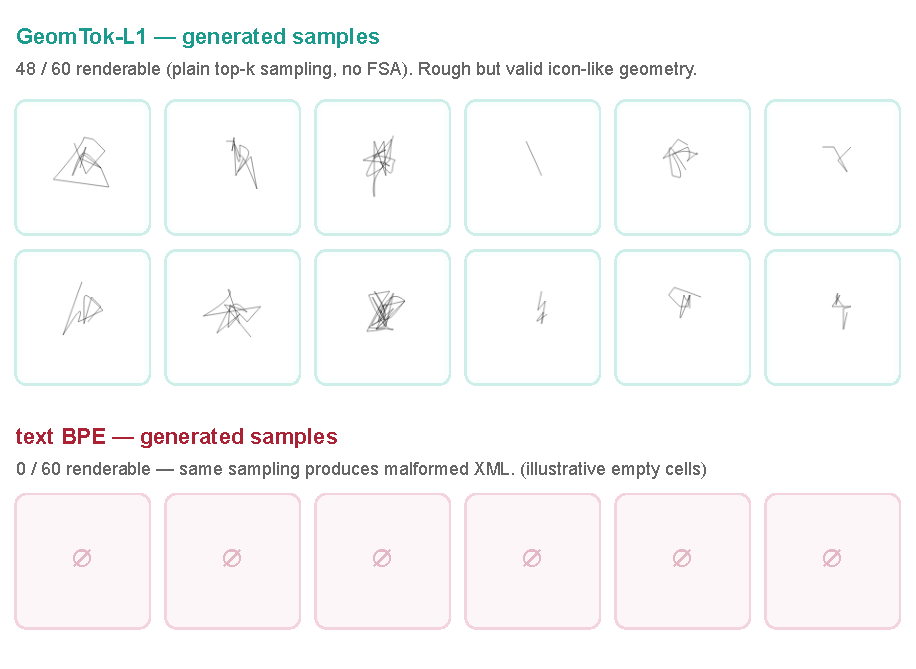
\includegraphics[width=\textwidth]{fig4_gen_samples.pdf}
\caption{Generated samples under identical plain sampling: GeomTok-L1 (48/60 renderable) vs.\ text BPE (0/60).}
\label{fig:gensamples}
\end{figure*}

\section{Controls and Retracted Claims}
\label{sec:controls}
We subjected each component to an adversarial control; three plausible claims did not survive, and we report them so the field does not repeat them.

\begin{itemize}
\item \textbf{``$7.6\times$ compression'' $\rightarrow$ retracted to $3.54\times$.} The $7.6\times$ figure compared against GPT-4's cl100k (100k vocab, not domain-trained)---a strawman. At matched 5{,}561 vocabulary the honest figure is $\mathbf{3.54\times}$.
\item \textbf{``Geometry-aware embedding initialization accelerates training'' $\rightarrow$ retracted.} A matched-norm control---random vectors rescaled to unit row-norm, with \emph{zero} geometric structure---closes the entire gap: random (default norm ${\sim}11.3$) val $4.51\rightarrow$ random-unit-norm $\mathbf{3.40}\approx$ geometry-structured $3.47$. The apparent benefit was a weight-tying embedding-\emph{norm} artifact, not geometry.
\item \textbf{``Adaptive quadtree coordinates'' $\rightarrow$ retracted for a uniform grid.} On 400 real icons (27{,}414 coordinates), at equal token count, a uniform $64\times64$ grid beat a curvature-adaptive quadtree decisively: mean error \textbf{1.78px vs.\ 14.75px}, SSIM \textbf{0.929 vs.\ 0.846}, ink-IoU \textbf{0.655 vs.\ 0.284} (Figure~\ref{fig:render}). Curvature-driven splitting starves straight content, which dominates real icons.
\end{itemize}

We also note that a saturated validity metric (100\% after a definition change) has no discriminative power, and that hand-crafted L2/L3 macros fire on ${\sim}0$--15\% of real icons. We argue this discipline---competing baselines, matched budgets, controls for confounds, and reporting what dies---is what this subfield most needs.

\begin{figure}[t]
\centering
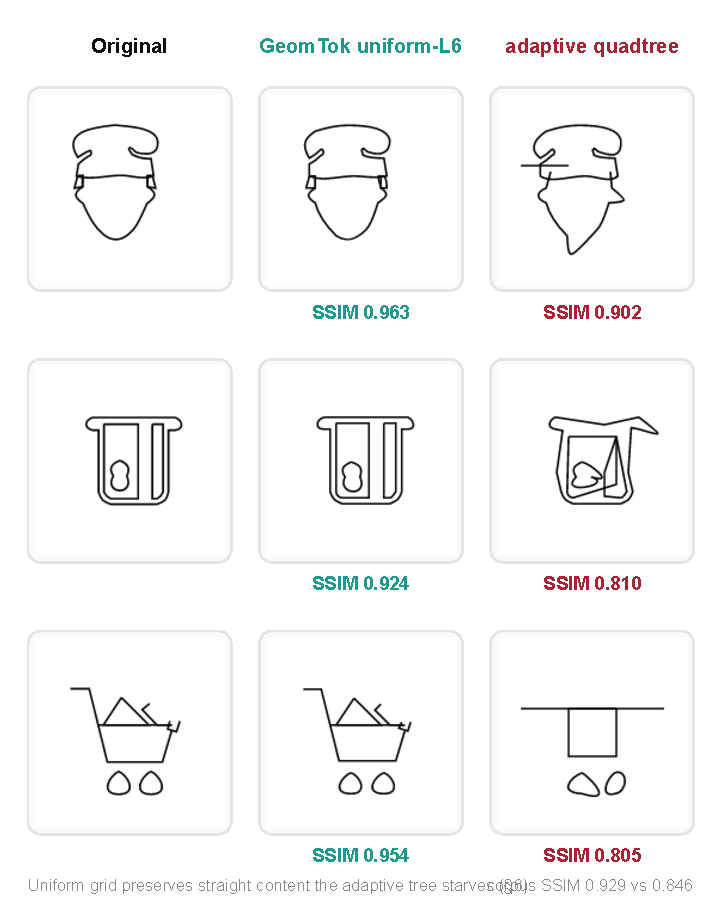
\includegraphics[width=\columnwidth]{fig3_render_panel.pdf}
\caption{Qualitative round-trip: original vs.\ uniform-L6 vs.\ adaptive-quadtree, with per-icon SSIM. The adaptive scheme warps straight content.}
\label{fig:render}
\end{figure}

\section{Conclusion}
The unit a model reads geometry in is not a free choice. On real vector graphics, in the small-model regime, geometric primitive tokens model and generate better than text---and, against intuition, better than the more-compressed learned-merge variant. We do not claim compression is irrelevant; we exhibit a controlled counterexample to the assumption that it predicts downstream quality, with an information-theoretic mechanism (merges trade token count for per-token entropy). We release GeomTok and GeomTok-Eval, with our negative-results ledger, to let the field measure this directly.

\section*{Limitations}
Experiments are CPU-scale: models up to 9.3M parameters on ${\sim}0.4$--1k icons, path-centric icons (and colored emoji as a second corpus), held-out NLL and a lightweight FID rather than large-model human-aligned generation. We therefore scope the model-level claims (\S\ref{sec:downstream}--\S\ref{sec:generation}) to the small-model, sample-efficient regime; we do not claim they transfer unchanged to 3--8B VLM scale. We note, however, that the substrate gap does \emph{not} shrink over the 0.9M--9.3M range (it widens then plateaus at 62 bits), which weakens the ``small-model artifact'' reading, though confirming persistence at 100M--1B remains the most important follow-up. Color/style and full SVG features (gradients, text, filters) are out of scope. The fixed-point codec overloads a token's meaning (position vs.\ scalar vs.\ count), an embedding confound we have not measured.

\textbf{The continuous-coordinate challenge.} The sharpest challenge to our premise is the continuous-coordinate camp \citep{ogezi2026cnm}: if coordinates are modeled as continuous values rather than discrete tokens, the notion of a tokenization ``unit'' dissolves. We test it directly. On an identical backbone and data, holding the coordinate \emph{input} continuous for both arms and varying only the output head---discrete cell-classification (4096-way) vs.\ continuous $(x,y)$ regression---we measure held-out, teacher-forced next-coordinate prediction error. The \textbf{discrete head is 18\% more accurate} (mean 35.7px vs.\ 43.3px; $n{=}2$ seeds): the categorical formulation is more robust than regression in this small-data regime. For our setting, dropping discrete tokens does not help; we make no claim about the large-data regime. \emph{Caveat:} our continuous arm is a minimal reimplementation (a Gaussian/MSE regression head), not a full continuous-modeling pipeline; we isolate only the output parameterization, holding everything else fixed.

% \section*{Acknowledgments} % add for [final]

\bibliography{references}

\appendix
\section{Reproducibility}
\label{sec:repro}
All numbers are produced by scripts against the public StarVector svg-icons benchmark; raw outputs are archived. The package installs as \texttt{geomtok} (\texttt{pip install -e .}); tests run via \texttt{pytest}. Datasets are pinned by revision (\texttt{starvector/svg-icons}, \texttt{starvector/svg-emoji}); the rasterizer is pinned (\texttt{resvg-py==0.3.2}) because render metrics depend on it. A full reproducibility record---pinned environment, dataset revision hashes, per-experiment split manifests, the model-config table, seeds, per-experiment wall-clock, determinism notes, and the experiment$\rightarrow$script$\rightarrow$result map---accompanies the (anonymized) release. The package is released under Apache-2.0, which the methodological/protocol framing requires. The full paper reproduces on a laptop CPU (Apple M4) in a few hours; no GPU required.

\end{document}
